\documentclass[11pt]{article}

\usepackage{amsmath,amssymb,amsthm,setspace,tabto,fancyhdr,sectsty,mathtools}
\usepackage{titleps}
\usepackage[left=1.00in,right=1.00in,top=0.75in,bottom=1.50in]{geometry}
\usepackage{graphicx}

% change this line
\graphicspath{ {assets/note4/} }

% start pdfinlimg (GPLv3, https://github.com/zerotoc/pdfinlimg/blob/master/pdfinlimg.sty)
\newcommand{\pdfinlimg}[5]{
\makebox[#1cm][l]{\immediate\pdfliteral{
  q
  #3 0 0 #4 0 0 cm
  #1 0 0 #2 0 0 cm
  0.885 0 0 0.885 0 0 cm 
  BI
  /W #3
  /H #4
  /CS /RGB
  /BPC 8
  /F [ /AHx /Fl ]
  ID
  #5>
  EI
  Q
}\vbox to #2cm{}}
}
% end pdfinlimg

% BEGIN PARAGRAPH STUFF
\usepackage[utf8]{inputenc}
\usepackage[english]{babel}
 
\setlength{\parindent}{4em}
% \setlength{\parskip}{1em}
\renewcommand{\baselinestretch}{1}
% END PARAGRAPH STUFF

% useful commands
\DeclarePairedDelimiter{\ceil}{\lceil}{\rceil}
\DeclarePairedDelimiter{\floor}{\lfloor}{\rfloor}

\newpagestyle{footers} {
    \sethead{}{}{}
    \setfoot{\small Intro to Crypto and Blockchain, Note \notenum}{\thepage}{\small Lin, Akhtar}
    \footskip = 45pt
}

\fancypagestyle{firstpage} {
    \vspace*{3\baselineskip}
    \footskip = 0pt
    \renewcommand{\headrulewidth}{6pt}
    \chead{\rule{\textwidth}{6pt} \vspace{20pt}\\}
    \lhead{\setstretch{1.05}\Large\fontfamily{lmdh}\selectfont
    Introduction to Cryptocurrencies and Blockchain 
    \\ Lin, Akhtar}
    \rhead{\huge \fontfamily{lmdh}\selectfont    Note \notenum}
    \lfoot{\small Intro to Crypto and Blockchain, Note \notenum}
    \rfoot{\small Lin, Akhtar}
}
    
\sectionfont{\Large\fontfamily{lmdh}\selectfont}

% for initial paragraph indent
\usepackage{indentfirst}

% UPDATE THIS FOR EVERY NEW NOTE
\newcommand{\notenum}{4}

\pagestyle{footers}

\begin{document}
    \thispagestyle{firstpage}
    \vspace*{2\baselineskip}
    
    
    \section*{Bitcoin Mechanics and Optimizations}
    
    After spending time abstracting away certain Bitcoin features to high level concepts, it's time to take a deeper dive into how Bitcoin works on a technical level. In this note, we will cover topics such as more advanced Bitcoin mechanics, scripting, optimizations we can run on the network. Through these topics, we hope to exemplify how Bitcoin's design philosophy has been made as simple, robust, and conservative as possible.
    
    \section*{Account vs Transaction Based Ledgers}
    
    Consider the notion of \textbf{account based ledgers}. There are certain cryptocurrencies such as Ethereum which maintain account based ledgers. Each address in Ethereum has an account, and for a user to check how many tokens they have, they simply add the inputs and subtract the outputs. The downside to this method is that the system must track every single transaction that has ever affected that one account. Scaling this to many thousands of users, this method could be a performance issue. One way to fix this huge amount of data is to 'prune' away old transaction history so that the user does not have to deal with old transaction data. This method has proven to be error-prone however, due to the additional block maintenance that is required. 
    
    On the contrary, Bitcoin is a \textbf{transaction-based ledger} (known as triple-entry accounting.) Users are always spending from previous outputs. As we mentioned in Note 2, UTXOs (unspent transaction outputs) can only be spent once, so Bitcoin has change addresses. By restricting UTXO usage and introducing the concept of change addresses, Bitcoin has a very efficient verification system. To determine how many tokens a user has, simply total the amounts associated with their recent UTXOs. The state of the Bitcoin network is only dependent on the most recent history. Bitcoin also supports joint payments, so that a transaction can have multiple inputs -- for example if Alice and Bob both want to pitch in to spend a total of 1.00 BTC. In practice, this feature is rarely used but is supported nonetheless.
    
    \section*{Contents of a Transaction}
    
    The contents of an actual transaction in Bitcoin can be split into three sections: the metadata, inputs, and outputs. 
    
   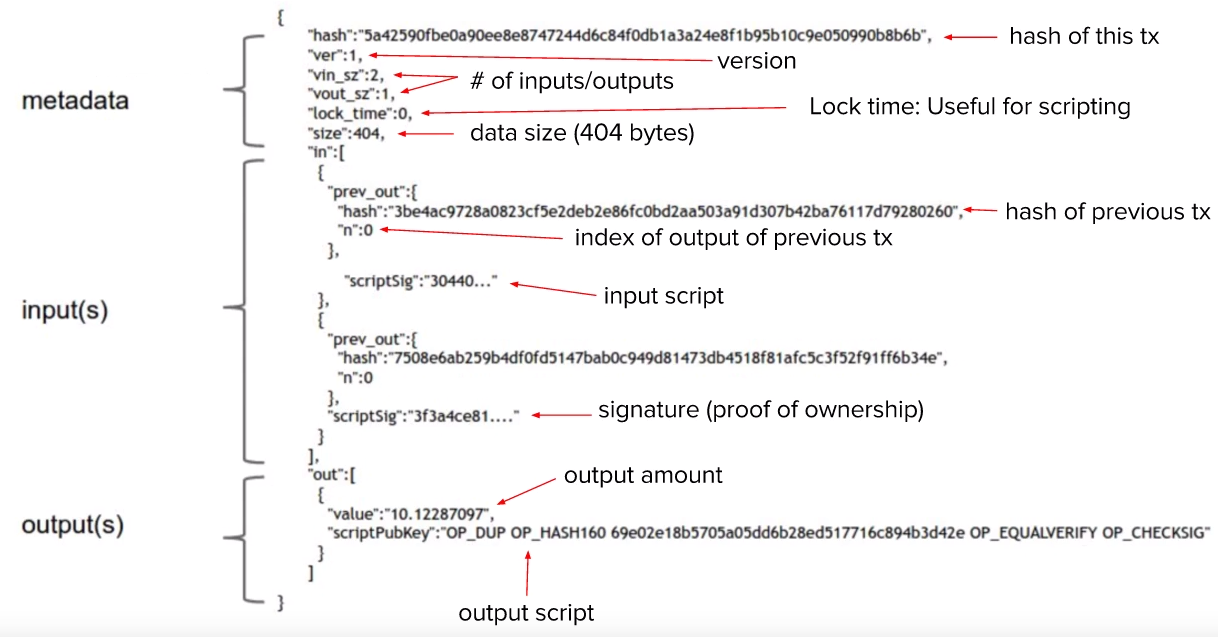
\includegraphics[scale=0.3]{transaction_contents}
   
   As seen above, a transaction folllows JSON structure. Metadata contains information such as the hash of the current transaction (often times referred to as the transaction ID), the version number (currently 1), the number of inputs and outputs, lock time, and data size.
   
   Inputs to the transaction include a hash of a previous unspent transaction, and an index specifying the output of the previous transaction from which the user is spending. Transaction outputs are ordered, so an index is required to identify specific outputs in a transaction. Inputs also need a signature as a cryptographic proof of ownership. 
   
   The outputs of a transaction include an output amount in BTC as well as an output script. The output script is what enables the parties associated with the transaction to claim their bitcoin later on, using a system called the Pay-to-PubkeyHash, which we will discuss later.
   
   \section*{Bitcoin Scripting}
   
   Previously we may have made the abstraction that transactions map input addresses to output addresses. In practice, these "addresses" we have been referring to are really scripts. By defining inputs and outputs through scripting, we can allow for the future extensibility of Bitcoin because scripting is such a low level feature that could potentially support many other future operations if needed. Recall that a signature proves the ownership of a public key, and that the Bitcoin address is a hash of the public key.
   
   $$Hash(PubKey)~==~Address~==~"PubKeyHash"$$
   
   Inputs and outputs are scripts that \underline{specify} these addressses, and sending money through transactions involves \underline{redeeming} previously unspent transaction outputs.
   
   So outputs in a transaction must be constructed in a way that tells the network:
   
   "This amount can be redeemed by a \underline{signature} from the owner of address X." 
   
   However, by the cryptographic property of preimage resistance, we know that we cannot find a public key given an address. What the transaction should really be saying is:
   
   "This amount can be redeemed by the \underline{public key} that hashes to address X, plus a \underlline{signature} from the owner of that public key."
   
   Only the owner of the public key would be able to produce the valid signature necessary to redeem the bitcoin from the output script.
   
   To make input scripts compatible with output scripts, we concatenate the input script to the output script, in that order. Input scripts are called \textbf{scriptSigs} and output scripts are called \textbf{scriptPubKeys}. This is because output scripts are specified by the senders of the transaction. Outputs need to know a provider -- a public key that hashes to the associated address, and makes sure that the signature matches.
   
  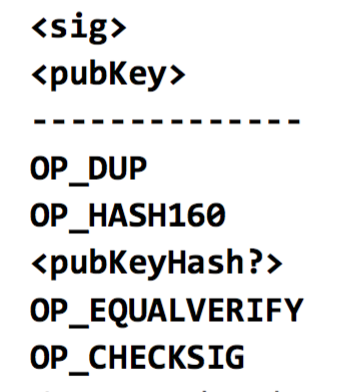
\includegraphics[scale=1]{output_script}
  
  In terms of code execution, scripts are run line by line, top to bottom. Notice in the diagram how the scriptSig is followed by the scriptPubKey because of the concatenation convention, and also because outputs need to know where the funds are coming from. 
  
  The Bitcoin scripting language, called \textbf{Script}, (the former is used frequently too) is a simple stack based language. There exists no support for loops, so the language is not Turing complete, but there exists native support for cryptography, making the language very specialized for its own needs. In fact, the entire signature verification process can be written in code as one instruction.
  
  Next, we present an example execution of the previously shown script. 

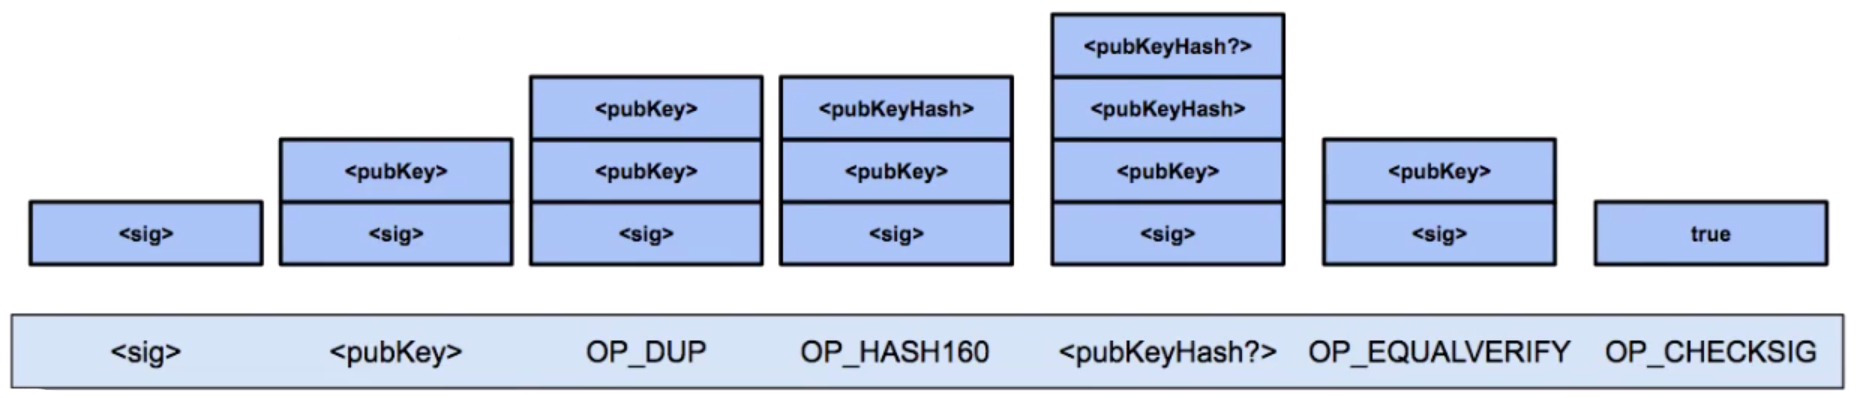
\includegraphics[scale=0.2]{script_execution} \\

 The first two steps are $<$sig$>$ and $<$pubKey$>$, so we push those to the stack in that order. Next, OP\_DUP simply duplicates the most recent instruction, so by the end of executing the third instruction, there are two $<$pubKey$>$'s. OP\_HASH160 hashes the topmost item, $<$pubKey$>$, into $<$pubKeyHash$>$, as the name implies. $<$pubKeyHash?$>$ is the address that redeemers of the output must hash their public key to. Next, in the instruction OP\_EQUALVERIFY, the script checks to see if $<$pubKey$>$ truly hashes to the address $<$pubKeyHash?$>$. The script then cross checks this with the signature, $<$sig$>$, in OP\_CHECKSIG, which returns true if the redeemer of this output is truly verified to spend from this output. In a nutshell, the script returns either true or false, depending on the legitimacy of the $<$sig$>$ and $<$pubKey$>$ that are passed in. 
 
 The output is saying: "This amount can be redeemed by
 \begin{enumerate}
     \item the $<$pubKey$>$ that hashes to the address $<$pubKeyHash?$>$
     \item plus a $<$sig$>$ from the owner of that $<$pubKey$>$, which will make the output script evaluate to true."
 \end{enumerate}
 
 \section*{Proof of Burn}
 
 One application of Bitcoin scripting is to implement something known as a \textbf{proof-of-burn}, which allows a user to prove the existence of some data in exchange for destroying bitcoin. There exists an instruction named OP\_RETURN that throws an error when reached, stopping code execution. By placing this instruction anywhere in an output script before the script returns either true or false, we can effectively make it so that no one can redeem that output. We have \textit{burned} that coin. Anything that exists after the OP\_RETURN will never be executed, but this allows us to prove its existence cryptographically.
 
 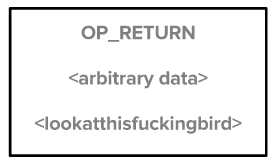
\includegraphics[scale=1]{burn_script} \\
 
 As seen in the sample script above, as long as we're willing to burn coin, we can prove the existence of anything at a particular point in time. This would be a word you coined, a hash of a document, music, your creative works, etc. If Alice stores a hash of a word she coined in the blockchain via proof-of-burn, she could then show everyone that "Alice coined word asdf at time 12345." Any data stored in this way in the blockchain is valid because blocks are timestamped. This is especially true when considering that the blockchain is provably immutable with honest actors. There have also been instances of burning bitcoin to bootstrap the value of other cryptocurrencies. To bootstrap an imaginary SuperAwesomeCoin, Super Awesome Bob could require users to burn bitcoin in order to get superAwesomeCoin. 
 
 \section*{Pay-to-PubKey-Hash vs Pay-to-Script-Hash}
 
 The previous example of requiring a public key and a signature in order to spend from a transaction output script is a use case of \textbf{P2PKH (pay-to-pubkey-hash)}, in which the vendor says "send your coins to the hash of this public key." This scheme represents the simplest and by far the most common case of transaction.
 
 However, for more complicated scripts, such as those which require multiple signature verification, P2PKH no longer works. For instance, if a merchant wants Alice to send coin payment to an output that allows the merchant to spend using multiple signatures, how would Alice know how to specify such a complicated script?
 
 The solution is to use a \textbf{pay-to-script-hash (P2SH)}. To clarify, consider following general cases:
 
 \begin{itemize}
     \item P2PKH: ``Send your coins to the hash of this \underline{public key}''
     \item P2SH: ``Send your coins to the hash of this \underline{script}. To redeem those coins, you must reveal the script that has the given hash and provide \underline{data} that will make the script evaluate to true.''
 \end{itemize}
 
 One of the most important improvements to the Bitcoin protocol since its inception, P2SH offloads the burden of complicated script writing to recipients of a transaction. When a merchant wants to receive payments from a customer, they do not want to burden the customer with writing a complicated script that could potentially differ between merchants. Instead, the merchant alone is responsible for writing a correct and secure script for the transaction. Likewise, the optimal customer experience is one in which the customer does not have to care about what the script actually is. They should not have to know anything about the company stores funds; customers should just have to create a transaction, pay, and leave.
 
 \section*{Merkle Trees}
 
 Let's take a deeper dive into the specifics of merkle trees, which we briefly touched upon in note 2. As review, merkle trees are inary trees of hash pointers. Blobs of transaction data are hashed together, then their hashes are hashed together, until one element remains --- the merkle root. (Note: Merkle trees are always full. If there are gaps, duplicate the last transaction to fill in the gaps.)
 
 Because outputs of cryptographic hash functions are unique, by \underline{second preimage resistance}, merkle trees are very efficient. Just from analyzing the merkle root, it is possible to prove that the merkle tree, a large string of data, contains a certain substring. To prove inclusion of data in the merkle tree, one must provide root data and intermediate hashes. Then, once hashing everything together in order, one would compare the final hash to the merkle root. To take this proof, one would need to find hash preimages that hash to valueus in the merkle tree. As discussed earlier, second preimage resistance makes faking proofs in merkle trees extremely difficult and practically impossible.

 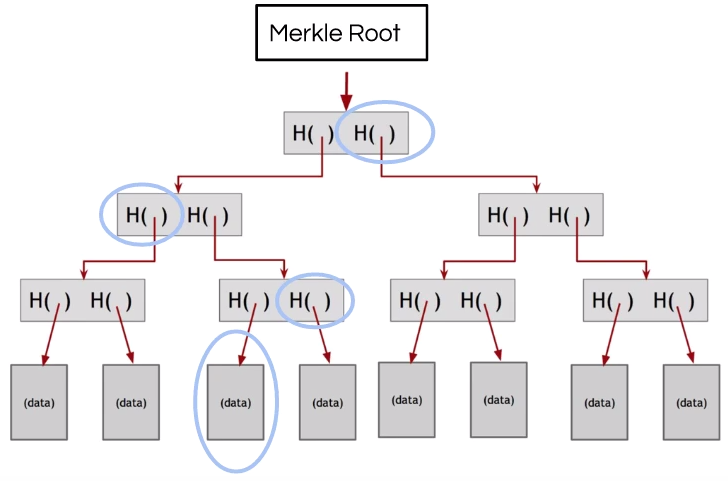
\includegraphics[scale=0.4]{merkle_proof} \\
 
 The figure above illustrates how one might prove the inclusion of a substring $data$, the circled leaf node. Provided the circled $data$, the proof proceeds as follows.
 
 \begin{enumerate}
     \item Hash $data$ and call it $H_{data}$
     \item Hash $H_{data}$ with the next intermediate hash (height 2)
     \item Continue hashing until we reach height 0
     \item Hashing the two hashes at height 0 results in $H_{root}$
     \begin{enumerate}
         \item If $H_{root}$ is the same as the merkle root, then we have proven the existence of $data$ within the merkle tree
         \item Else, the proof failed and the merkle tree does not contain $data$
     \end{enumerate}
 \end{enumerate}
 
 \section*{Merkle Trees --- Bitcoin Construction}
 
 There are two main hash structures in Bitcoin. The blockchain is a hash chain of blocks; the blocks are linked together and based off of each other. They are tamper evident because changing one block changes its hash, which mismatches with the next block's hash of the previous block. Merkle trees exist within blocks and are a way of storing transactions. Changing data within a merkle tree changes its hashes, ultimately bubbling up and changing the merkle root. Changing the merkle root in turn changes the hash of the block it's contained in, invalidating the block.
 
 \section*{Merkle Trees --- Mining, In More Detail}
 
 Previously, we explained for simplicity that for every block, miners hashed together the merkle root, the previous block's hash, and a nonce (varied value) to find a number that is below a certain target value. There are actually two nonces: one in the block header as mentioned, and one in the coinbase transaction, the transaction that is created by and paid out to the miner. Changing the nonce in the coinbase transaction changes the hash of the coinbase transaction, ultimately changing the merkle root.
 
 The reason why there are two nonces is to increase difficulty for the miner. The block header nonce is 32 bits by itself. A modern ASIC such as the Antminer S9 can hash at 14 TH/s. A simple calculation shows that it takes just 0.00031 seconds to compute all the possible combinations in the block header nonce. $2^{32} / 14,000,000,000,000 = 0.00031 \text{~seconds}$. A miner with the right hardware can exhaust all nonce combinations 3260 times per second. Therefore, it is imperative to change the merkle root by including the coinbase transaction nonce.
 
 A common strategy is to increment the coinbase nonce, and then run through all block header nonce combinations. A less efficient strategy is to increment the block header nonce, and then run through all combinations for the coinbase nonce. This is because changing the coinbase nonce changes the merkle root, and the change must propagate up the tree, wasting precious hash time. (Propagating up the merkle tree takes $\theta(\log N)$ time, whereas calculating a hash takes $\theta(1)$ time.) We want to minimize the time spent calculating new merkle tree hashes, so change the coinbase transaction as little times as possible.
 
 \section*{SPV --- Simplified Payment Verification}
 
 The current size of Bitcoin's blockchain is 122.7 gigabytes and growing. Miners, or ``full nodes'', are required to save the entire blockchain, but for the average user, such a requirement is not feasible if the aim is mass adoption. Enter \textbf{SPV (Simplified Payment Verification) nodes}, or ``thin'' clients. These nodes are designed to be lightweight, as their name implies. They only store the pieces of data needed to verify transactions that concern them, thus relieving the necessity to store the entire blockchain. Nearly all nodes in the Bitcoin network are SPV nodes because users are discouraged by the enormous download size. Those that do run full nodes exchange large amounts of storage and a high bandwidth for a shot at the block reward.
 
 \section*{Double Spend --- Example}
 
 To gain further intuition on Bitcoin consensus, it is important to understand how double spending works. Previously we defined a double spend as a circumstance in which a party successfully spends the \underline{same} money more than once. For example, if Alice wants to purchase something from Bob for 1.00 BTC, she can double spend and send 1.00 BTC to Bob and also herself. Double spends are possible when a party gains more than 50\% of the network's hash power. Under the hood, there is a fairly involve process that results in the double spend.
 
 \section*{Double Spend --- Confirmations}
 
 Before going into the technical details of double spending, we will look at a more basic concept. A \textbf{confirmation} is the number of blocks created on top of the block a transaction is in. It is simply calculated by subtracting 1 from the block depth, since we want the most recent block to have 0 confirmations. 
 
  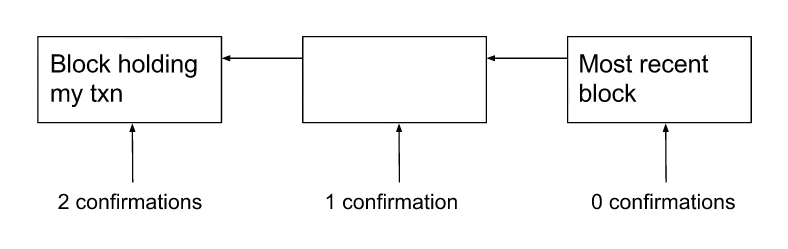
\includegraphics[scale=0.5]{confirmations} \\
  
  Because of the difficulty of finding the proof-of-work for each block, confirmations are especially important because they roughly determine the security of transactions. In order to double spend a transaction, one must calculate the proof-of-work for each block until their fork of the blockchain is the longest. In the diagram above, one would have to calculate 3 different proofs-of-work starting with the block with 2 confirmations, to reach the same height as the most recent block. This is also assuming that the double spender has a significantly higher hash rate than that of the rest of the network, which is working on the original blockchain.
  
  What about transactions with no confirmations at all? Suppose Bob does not wait for \textit{any} confirmations on Alice's transaction. He simply checks that the transaction from Alice is valid, and \textit{immediately} sends Alice the product he is selling. Since there are no confirmations on Bob's transaction, Bob is vulnerable to a \textbf{race attack}. Alice can send a competing transaction to herself at the same time she sends Bob the legitimate transaction. Alice can then broadcast the transaction to the entire network. The false, conflicting transaction Alice sends is propagated much faster than the single transaction she sends to Bob, so there is a high likelihood that one of the Alice's conflicting transactions will be mined into a block and accepted by the network as genuine. Alice can also increase the block fee for the transaction to provide more incentive for miners to include the illegitimate transaction into their blocks. In this case, merchant Bob's waiting for 0 transactions makes him vulnerable to anyone that wants to steal goods. 
  
  On the other hand, in the case that Bob waits for more than 1 confirmation ($z$ confirmations), Alice can still double spend, but the process is more involved. Say Alice sends Bob a transaction, and Bob waits $z$ confirmations before he sends the goods to Alice. In order to double spend on Bob, Alice must mine on her own private chain, one that does not have the transaction that sent bitcoin from Alice to Bob; Alice can send the same transaction to herself instead. She builds up an illegitimate transaction history such that she sends money to herself rather than to Bob. After mining $z$ blocks, and making sure that her chain is longer than any other chain, Alice can broadcast her chain (preferably after she receives the goods from Bob). The network will adopt Alice's chain over the previous chain because it is longer in length. In fact, it is proven that if Alice has greater than 50\% of the total hash power, then she can always have a longer, illegitimate chain. \\ \\
 
   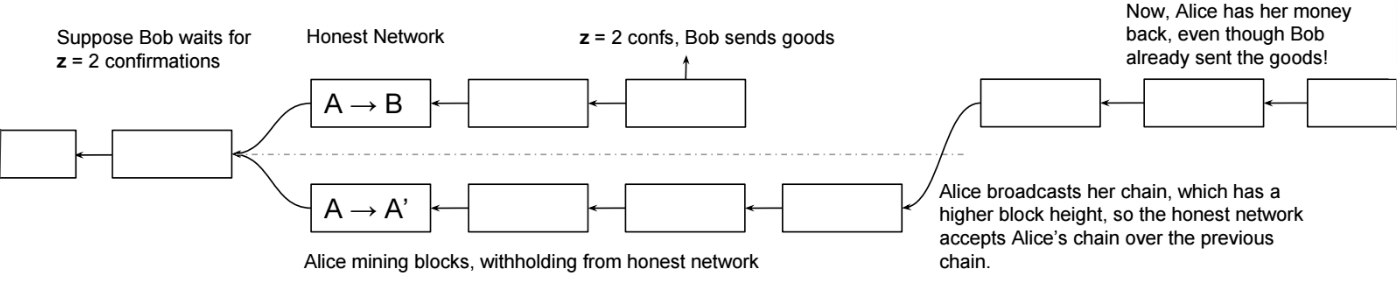
\includegraphics[scale=0.3]{z_confirmation} \\
   
   \section*{Double Spend --- Security}
   
   Now we'll model our assertions regarding double spending and hash power using mathematics:
   
   Suppose Bob waits for $z$ confirmations before sending his goods over to Alice. Alice has $h_A$ hash power, and the honest network has $h_H$ hash power. The total network hash power is then $h_A + h_H$. 
   
   The probability, $p$, of the honest network finding the next block is simply the proportion of hash power the honest network controls:
   
   $$p = \frac{h_H}{h_A + h_H} $$
   
   The probability, $q$, of Alice finding the next block is the complement of $p$. We calculate it as follows:
   
   \begin{equation*}
       \begin{split*}
           q = 1-p &= 1 - \frac{h_H}{h_A + h_H} \\
           &= \frac{h_A}{h_A + h_H}
       \end{split*}
   \end{equation*}
   
   Consider the scenario in which the honest network mines $z$ blocks on top of Alice's transaction to him. Bob sees that there are $z$ confirmations, and then he sends the goods over to Alice. In the meantime, Alice has been hard at work mining on her own chain ever since sending her transaction over, in hopes of double spending on Bob. The expected number of blocks Alice would have mined after the $z$ confirmations is equal to:
   
   $$\lambda = z(\frac{q}{p})$$
   
   If we model this as a Poisson distribution, because we have discrete events each corresponding to a probability, we can show that the probability that Alice generates $k$ blocks is:
   
   $$p_A(k) = \frac{\lambda^k e^{-\lambda}}{k!}$$
   
   Now the question is: What is the probability Alice can mine enough blocks in secret to successfully broadcast her chain with the double spend? In other words, what is the probability that Alice can produce a longer chain than the honest network? 
   
   To solve this, first consider the related problem of Alice trying to catch up to a chain that is $j$ blocks ahead of Alice's own chain. The corresponding question is: What is the probability that Alice will ever catch up given an unlimited number of trials? It is also important to consider that the honest network is continuously mining their blocks on their chain, while Alice works maliciously on the side. This problem is actually an instance of the \textbf{Gambler's Ruin} problem, which has the following probability for Alice catching up if she is $j$ blocks behind: 
   
   \[ p_c(j) = \begin{cases} 
      1 & q \geq p \text{ OR } j < 0 \\
      \big(\frac{q}{p}\big)^j & q < p
   \end{cases}
   \]
   
   Combining these two probabilities, we can compute the probability that Alice can catch up after $z$ blocks mined on the honest chain. Consider the case when Alice mines $k$ blocks. This means that the honest chain is $z-k$ blocks ahead of Alice. We sum over all possible values of $k$:
   
   \begin{equation*}
       \begin{split}
           &\Sigma_{k=0}^\infty p_A(k) \cdot p_C(z-k) \\
           = &\Sigma_{k=0}^\infty \frac{\lambda^k e^{-\lambda}}{k!} \cdot  \left\{
    \begin{array}{ll}
      1  & k > z \\ 
      \big(\frac{q}{p}\big)^{z-k} & k \leq z \\
    \end{array}
  \right.
       \end{split}
   \end{equation*}
   
   
    
    
    
    
    
    
    
    
    
    
    
    
    
    
    % BEGIN KEY TERMS
    \newpage
    \thispagestyle{firstpage}
    \vspace*{2\baselineskip}
    \section*{Key Terms}
    \noindent A collection of terms mentioned in the note which may or may not have been described. Look to external sources for deeper understanding of any non-crypto/blockchain terms.
    \begin{enumerate}
        % edit within here
        \item \textbf{VOCAB WORD} --- Definition. % format
    \end{enumerate}
    % END KEY TERMS
\end{document}